\documentclass[a4paper,11pt,fleqn]{article}%fleqn pour aligner les equations à gauche
\usepackage{../../Styles/Exercice}


\newcommand{\chnum}{Chapitre 16}
\newcommand{\chtitle}{Lentilles minces convergentes}
\newcommand{\dtype}{Exercices}

\begin{document}
\maketitle
\begin{multicols}{2}
\section{Les appareils imageurs}
L'appareil photographique et le vidéo-projecteur sont deux appareils qui utilisent un ensemble de lentilles modélisables par une lentille mince convergents de distance focale $f'$.\\
On considère un vidéo-projecteur pour lequel \uline{l'objet est à une distance comprise entre $f'$ et $2f'$ de la lentille. le grandissement est tel que $|\gamma|>1$}.\\
On considère un appareil photographique pour lequel \uline{l'objet est à une distance supérieure à $2f'$ : le grandissement est tel que $|\gamma|<1$.}\\
\textbf{Question compacte : Vérifier graphiquement les informations soulignées dans le texte}\\
\textbf{Question détaillée :}
\begin{enumerate}
    \item Schématiser une lentille convergente, en plaçant sur le schéma le centre optique $O$, et les foyers objet $F$ et image $F'$.
    \item \begin{enumerate}
        \item Placer un segment fléché $AB$ sur l'axe optique à une distance comprise entre $f'$ et $2f'$ du centre optique de la lentille. Construire son image.
        \item Placer un segment $AB$ de même taille sur l'axe optique à une distance supérieure à $2f'$. Construire son image.
    \end{enumerate}
    \item Comparer la taille des deux images obtenues à la question \textbf{2.} à celle de l'objet.
    \item Vérifier graphiquement les informations en italique dans le texte.
\end{enumerate}

\section{Où est la lentille ?}
Sur le schéma ci-dessous sont indiquées la position de l'objet et celle de l'image.
\begin{center}
	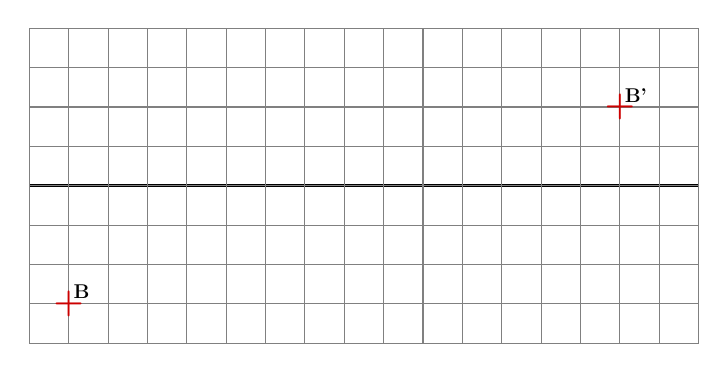
\begin{tikzpicture}[scale=.5, transform shape]
    \draw[very thick] (0,0) -- (17,0);
    \draw[gray] (0,-4) grid (17,4);
    \node[red!80!black] (b) at (1,-3){\Huge \textbf{+}};
    \node[above right] (B) at (1,-3){\Large\textbf{B}};
    \node[red!80!black] (b') at (15,2){\Huge \textbf{+}};
    \node[above right] (B) at (15,2){\Large\textbf{B'}};
    \end{tikzpicture}
\end{center}

\begin{enumerate}
    \item Où est située la lentille ? Reproduire le schéma et la dessiner dessus.
    \item Déterminer la distance focale de cette lentille.
\end{enumerate}

\section{Accommodation de l'\oe il}
Pour que les images soient situées sur la rétine, le cristallin change de forme : c'est l'accommodation. Le schéma suivant est le modèle de l'\oe il réduit. Sur ce schéma, les distances et les proportions ne correspondent pas à celles de l'\oe il réel.
\begin{center}
    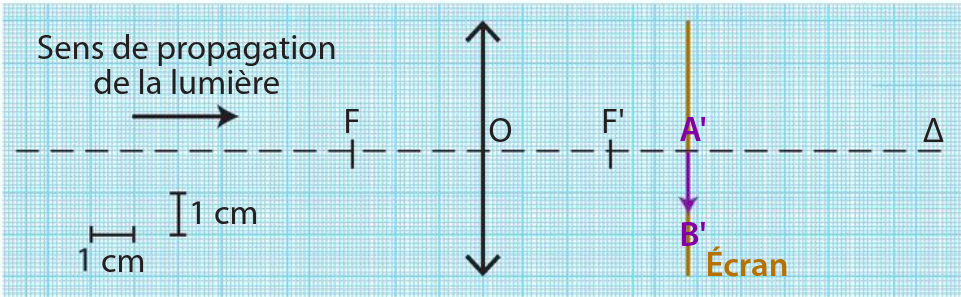
\includegraphics[width=\linewidth]{Ressources/2GT_C16_ExOeil.png}
\end{center}
\begin{enumerate}
    \item Reproduire et compléter le schéma pour trouver la position de l'objet $AB$ donnant une image $A'B'$ sur l'écran.
    \item Rapprocher l'objet $AB$ de \SI{3}{cm} de la lentille et trouver les nouvelles positions des foyers objet $F$ et image $F'$ pour que l'image $A'B'$ se forme à nouveau sur l'écran.
    \item Quelle caractéristique de l'\oe il est modifiée lors de cette accommodation ?
\end{enumerate}

\section{Les lentilles liquides}
\noindent \begin{minipage}{.99\linewidth}
    \textbf{Document 1 : Principe de fonctionnement}\\
    Les lentilles liquides sont constituées de deux fluides non miscibles (eau-huile) placés dans une capsule.\\
    L'adhérence des fluides sur les parois de cette capsule varie lorsqu'une tension électrique est appliquée sur ces parois, ce qui entraîne une déformation de la surface de contact eau/huile sont la courbure varie. La lentille liquide comporte alors comme une lentille mince convergente dont la distance focale change en fonction de la tension électrique appliquée. L'image réelle de l'objet photographié se forme sur un capteur situé à une distance fixe de la lentille.
\end{minipage}\\

\noindent \begin{minipage}{.99\linewidth}
    \textbf{Document 2 : Vue en coupe d'une capsule}\\
    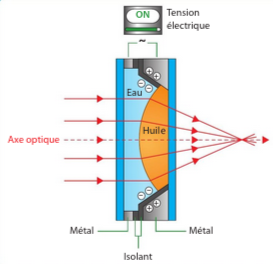
\includegraphics[scale=1.3]{Ressources/2GT_C9_Ex_Fig1.png}
\end{minipage}

\begin{enumerate}
    \item \begin{enumerate}
        \item Expliquer comment on fait varier la distance focale d'une lentille liquide.
        \item Comment nomme-t-on le point d'intersection des rayons lumineux ayant traversé al lentille liquide (\textbf{Doc. 2}) ?
        \item Citer un point commun entre le fonctionnement d'une lentille liquide et celui de l'\oe il.
    \end{enumerate}
    \item  On repère sur le capteur la position de l'image $A'B'$ d'un objet $AB$ placé à \SI{60}{mm} de la lentille. La taille de l'image est de \SI{1,5}{mm} et celle de l'objet est de \SI{15}{mm}. Par application du théorème de Thalès, calculer la distance $OA'$.
    \item \begin{enumerate}
        \item Faire un schéma de la lentille, de l'objet et de con image, puis repérer la position du foyer image $F'$. Choisir l'échelle suivante : \SI{1}{cm} sur le schéma représente \SI{3}{mm} dans la réalité.
        \item Mesurer la distance focale.
    \end{enumerate}
    \item \begin{enumerate}
        \item L'image se formant  toujours sur le capteur, calculer sa nouvelle taille lorsque l'objet se rapproche à \SI{30}{mm} de la lentille.
        \item Pour que l'image se forme toujours sur le capteur, la distance focale est maintenant \SI{5,0}{mm}. Retrouver par une construction graphique la taille de l'image calculée précédemment, en utilisant la même échelle.
    \end{enumerate}
\end{enumerate}
\end{multicols}
\end{document}